
\chapter{Technické pozadie výskumu} 
\label{kap:technické_pozadie}
\pagestyle{fancy}
\fancyhf{}
\fancyfoot[CE,CO]{\thepage}
\renewcommand{\footrulewidth}{1pt}
\lhead{Medicínske pozadie výskumu}

Snahou hĺbkových kamier je zachytiť okrem informácii o farbe prostredia aj informáciu o hĺbke priestoru. V praxi to znamená, že sa transformuje 3D priestor do 2D priestoru. Táto informácia je uchovávaná v matici, ktorá je nazývaná hĺbková mapa. Spôsob vytvárania hĺbkovej mapy kamerou závisí od použitej technológie. Medzi základné spôsoby patrí stereo-vízia, snímanie štrukturovaným svetlom (SLS) a meranie doby letu (TOF).

\section{Skenovanie v reálnom čase pomocou \mbox{RGB-D} senzorov}

Skenovanie dynamických objektov v reálnom čase je v centre záujmu už niekoľko rokov. V posledných rokoch sa hĺbkové snímače stavajú súčasťou riešenia rôznych technických problémov. Existuje viacero spôsobov, ktoré dokážu kvalitne rekonštruovať objekty v reálnom čase. Väčšinou sú to komplexné riešenia, ktoré sú cenovo nedostupné pre bežných užívateľov. Avšak existuje aj niekoľko cenovo dostupných RGB-D senzorov, ktoré môžu byť použité na 3D snímanie a rekonštrukciu v reálnom čase. V ďalšej časti sú opísané aktuálne riešené problematiky 3D skenovania dynamických objektov v reálnom čase. 

\newpage
\subsection{Viac-pohľadové 3D snímanie a analýza pre rekonštrukciu vysoko kvalitných mračien bodov}

V článku \textit{Multiview 3D Sensing and Analysis for High Quality Point Cloud Reconstruction} sa autori zaoberajú rekonštrukciou mračien bodov pomocou viacerých ToF kamier. 
V prvom kroku riešili kalibráciu,ktorá je kritickým krokom v celom procese. Využili metódu kalibrácie pomocou planárneho kalibračného vzoru (šachovnice), kde identifikovali rotačné a translačné parametre pre jednotlivé kamery. 

\begin{figure}[h]
	\centering
	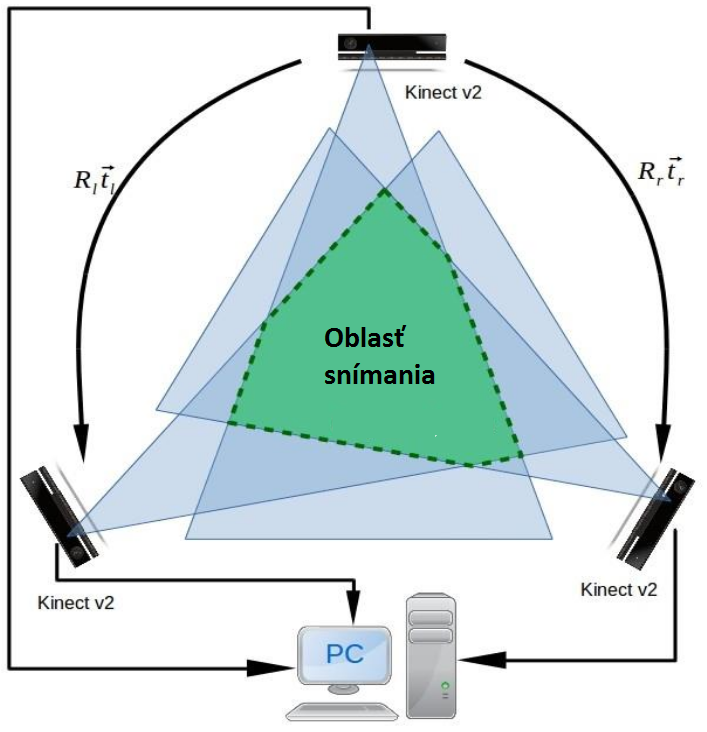
\includegraphics[width=0.55\textwidth]{figures/resers_m.png}
	\caption{Rekonštrukčný systém pozostávajúci z troch senzorov Kinect v2.}
	\label{fig:resers:m}
\end{figure}

V práci používali trojicu kamier Kinect v2, ktoré pracovali v sekvenčnom režime. Tým sa vyhli multi-kamerovej interferencii. Kvalita hĺbkovej mapy je kľúčovým faktorom pri tvorbe a rekonštrukcii modelu. Ak sa v nej vyskytnú chyby, tie sa potom prenášajú do mračna bodov. Túto hĺbkovú mapu filtrovali použitím bilaterálneho filtra (BF), \textit{Weight Median} filtra (WM) a \textit{Radius Outlier Removal} filtra (ROR). Vplyv filtračných metód na hĺbkovú mapu je zobrazený na obr. \ref{fig:resers:5}. Okrem toho tiež použili \textit{Weighted  Inter-Frame  Average} filter (WIFA), ktorý pracuje so sériou hĺbkových máp. Ten odstraňuje priestorový šum, ale výrazný pohyb robí aplikáciu WIFA nevhodnou pre vysoko dynamické scény.

\begin{figure}[H]
	\centering
	\begin{subfigure}[b]{0.24\textwidth}
		\centering
		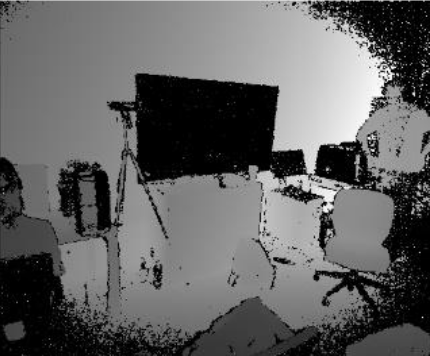
\includegraphics[width=\textwidth]{figures/resers_n.png}
		\caption{}
		\label{fig:resers:n}
	\end{subfigure}
	\hfill
	\begin{subfigure}[b]{0.24\textwidth}
		\centering
		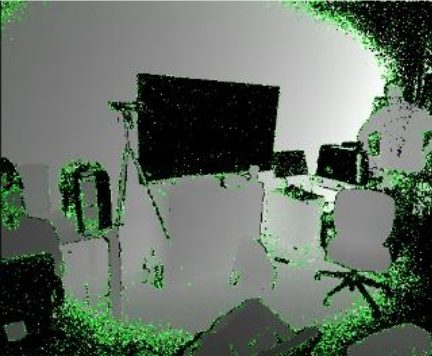
\includegraphics[width=\textwidth]{figures/resers_o.png}
		\caption{}
		\label{fig:resers:o}
	\end{subfigure}
	\hfill
	\begin{subfigure}[b]{0.24\textwidth}
		\centering
		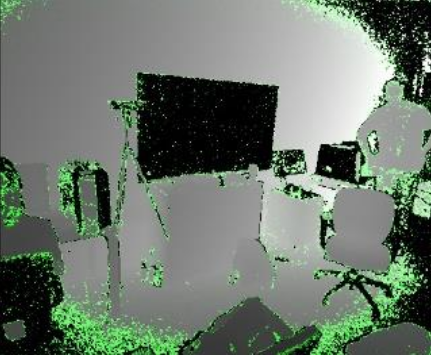
\includegraphics[width=\textwidth]{figures/resers_p.png}
		\caption{}
		\label{fig:resers:p}
	\end{subfigure}
	\hfill
	\begin{subfigure}[b]{0.24\textwidth}
		\centering
		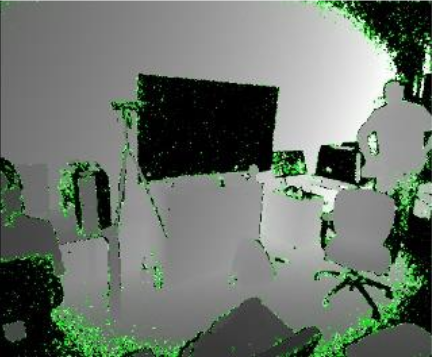
\includegraphics[width=\textwidth]{figures/resers_q.png}
		\caption{}
		\label{fig:resers:q}
	\end{subfigure}
	\caption{Výsledky filtrácie hĺbkej mapy, kde zelená farba predstavuje rozdiely medzi prístupmi filtrácie: (\textbf{a}) Vstupná hĺbková mapa. 
		(\textbf{b}) Filtrácia pomocou BF.
		(\textbf{c}) Filtrácia pomocou BF + WM.
		(\textbf{d}) Filtrácia pomocou BF + WM + ROR }
	\label{fig:resers:5}
\end{figure}


Mračná bodov zo všetkých Kinect v2 sa následne spájajú do jedného mračna, čím sa vytvorí jednotná uniformná reprezentácia snímanej scény. Algoritmus rekonštrukcie sa používa na vytvorenie vernej a podrobnej reprezentácie povrchu skenovaných tvarov. V ďalšej fáze sa generuje trojuholníková sieť zachyteného 3D objektu. 


\begin{figure}[H]
	\centering
	\begin{subfigure}[b]{0.32\textwidth}
		\centering
		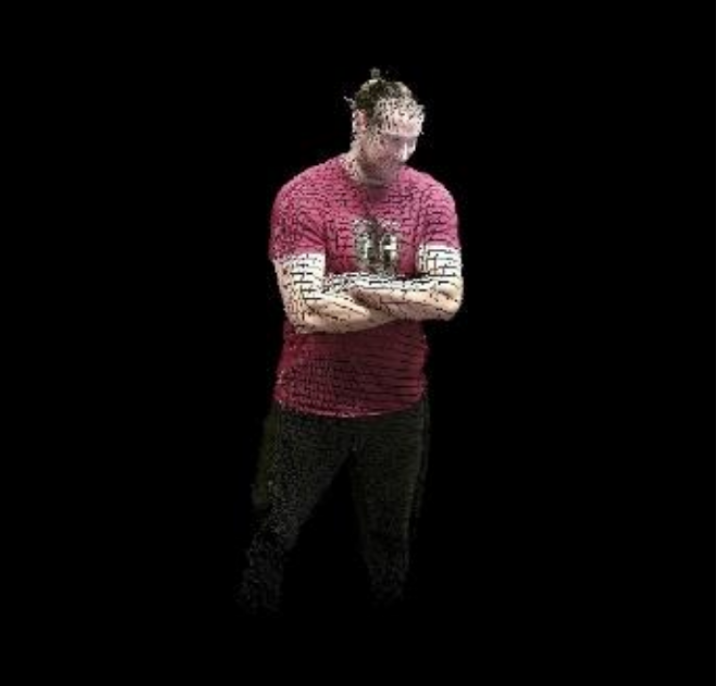
\includegraphics[width=\textwidth]{figures/resers_r.png}
		\caption{}
		\label{fig:resers:r}
	\end{subfigure}
	\hfill
	\begin{subfigure}[b]{0.315\textwidth}
		\centering
		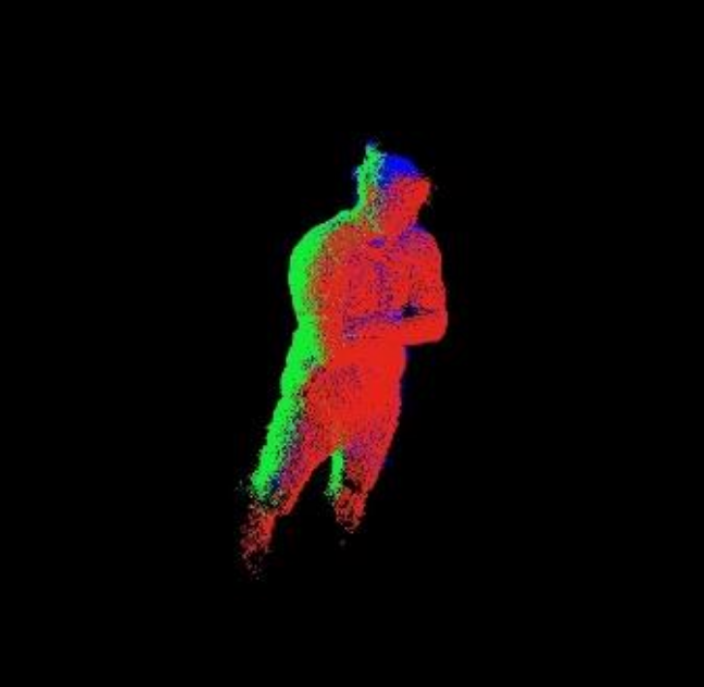
\includegraphics[width=\textwidth]{figures/resers_s.png}
		\caption{}
		\label{fig:resers:s}
	\end{subfigure}
	\hfill
	\begin{subfigure}[b]{0.32\textwidth}
		\centering
		
\includegraphics[width=\textwidth]{figures/resers_t.png}
		\caption{}
		\label{fig:resers:t}
	\end{subfigure}
	\caption{Rekonštrukcia scény z troch snímačov Kinect v2:
		(\textbf{a}) Mrak fúzovaných bodov generovaný každým snímačom Kinect.
		(\textbf{b}) Farebné oddelenie fúzovaných mračien bodov pre každú kameru.
		(\textbf{c}) Trojuholníková sieť vytvorená zo spojených mračien bodov.}
	\label{fig:resers:6}
\end{figure}

V článku sa zamerali aj na meranie rýchlosti spracovania filtrácie. Pre prácu použili CUDA paralelné spracovanie na grafickej karte GeForce 780GTX. 
Meranie rýchlosti spracovania jednotlivých častí algoritmu sa vykonávalo na 400 hĺbkových mapách. Priemerný čas filtrácie so sieťovou rekonštrukciou trval $14.19ms$. 

Autori predstavili návrh multi-kamerovej spolupráce 3 ToF snímačov značky Kinect v2. Bol opísaný spôsob kalibrácie a registrácie mračien bodov z jednotlivých kamier. Zároveň sa zamerali aj na filtráciu a trojuholníkovú rekonštrukciu snímaných objektov, pričom testovali rýchlosť spracovania.

\section{Disparitná a hĺbková mapa}

Výstupný obraz zachytávajúci vzdialenosť je závislý od použitej technológie snímania.
Výstupom kamery je buď disparitná alebo hĺbková mapa.
Disparita zachytáva relatívnu vzdialenosť navzájom si odpovedajúcich bodov v stereo-páre
obrazu. Pri vytváraní disparity sa predpokladá s nulovou vertikálnou paralaxou. K výpočtu je teda potrebné mať dvojicu obrazov v epipolárnej rovine. Ak teda bod vľavom obraze na pozícii [10,0] odpovedá v pravom obraze bodu [100,0], tak hodnota disparity je 90. Pri výpočte sa jeden obraz zo stereo-páru berie ako referenčný.  
V disparitnej mape každý pixel nesie informáciu o disparite. Zobrazením vzniká obraz v odtieňoch sivej, ktorý vytvára ucelenú informáciu o priestore.

Disparitná mapa je vždy vytváraná pre jeden obraz z dvojice, ktorej pozícia bodu sa berie ako referencia. Takáto mapa je už pre aplikáciu v stereovízií užitočná, pretože je z nej možné odlíšiť rozloženie snímanej scény. Neposkytuje však informáciu o reálnej vzdialenosti.

Hĺbková mapa je taktiež šedo-tónový obraz, ktorý zachytáva informáciu o absolútnej
vzdialenosti snímanej scény od kamery. 

\section{Princíp činnosti RGB-D kamier}
\label{sec:rgbd:principles}
RGB-D kamery sú optické snímače, ktoré zachytávajú hĺbkovú informáciu scény. Existuje viacero metód, ktorými tieto zariadenia pracujú. V tejto časti práce sú opísané najčastejšie používané metódy pre meranie hĺbky.  

\begin{itemize}
	\item \textbf{stereo-vízia:} ZED, Intel RealSense d415, stereo RGB
	\item \textbf{snímanie štrukturovaným svetlom (SLS):} Intel RealSense SR300 
	\item \textbf{meranie času doby letu (TOF):} Microsoft Kinect v2 
\end{itemize}

\newpage
\subsection{Stereovízia}

Metóda stereovízie je založená na synchronizovanom snímaní scény pomocou viacerých párov kamier (RGB alebo IR), ktoré sú voči sebe vzájomne posunuté. Najčastejšie rozloženia kamier sú Toe-In a Off-Axis, ktorá je znázornená na obr. \ref{fig:stereovizia}. Výstupom je farebný obraz scény zosnímanej z viacerých perspektív.

\begin{figure}[h]
	\centering
	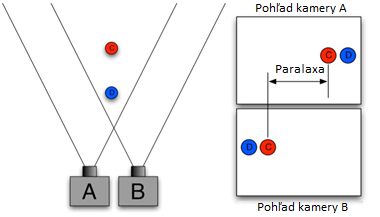
\includegraphics[width=0.6\textwidth]{figures/stereovizia.png} 
	\caption{Princíp stereovízie s Off-Axis nastavením kamier.}
	\label{fig:stereovizia}
\end{figure}

Na základe rozdielu z týchto dvoch perspektív a známych vonkajších parametrov stereo-kamerovej sústavy je možné dopočítať hĺbkový obraz. Hlavnou nevýhodou je vysoká výpočtová náročnosť algoritmu a cena kvalitných snímacích RGB senzorov. Taktiež je tento systém náchylný na meniace sa svetelné podmienky, čo následne vyžaduje farebnú kalibráciu jednotlivých kamier. Výhodou je nulová vzájomná interferencia.

\subsection{SLS snímače}
\label{sec:sls}
Structured Light Sensors (SLS) snímače sú zložené z projektora štrukturovaného svetla a snímača. Projektor aktívne osvecuje scénu so špeciálne navrhnutým 2D vzorom, častokrát priestorovo modulovaným svetlom. Kamera následne sníma osvetlenú scénu a získané dáta porovnáva s projektovaným vzorom. Ak je scéna planárna, snímaný vzor sa zhoduje s referenčným vzorom. Ak sú však v scéne povrchové variácie, geometrický tvar povrchu narúša projektované štrukturované svetlo. To sa následne nebude zhodovať s projektovaným vzorom.

\begin{figure}[H]
	\centering
	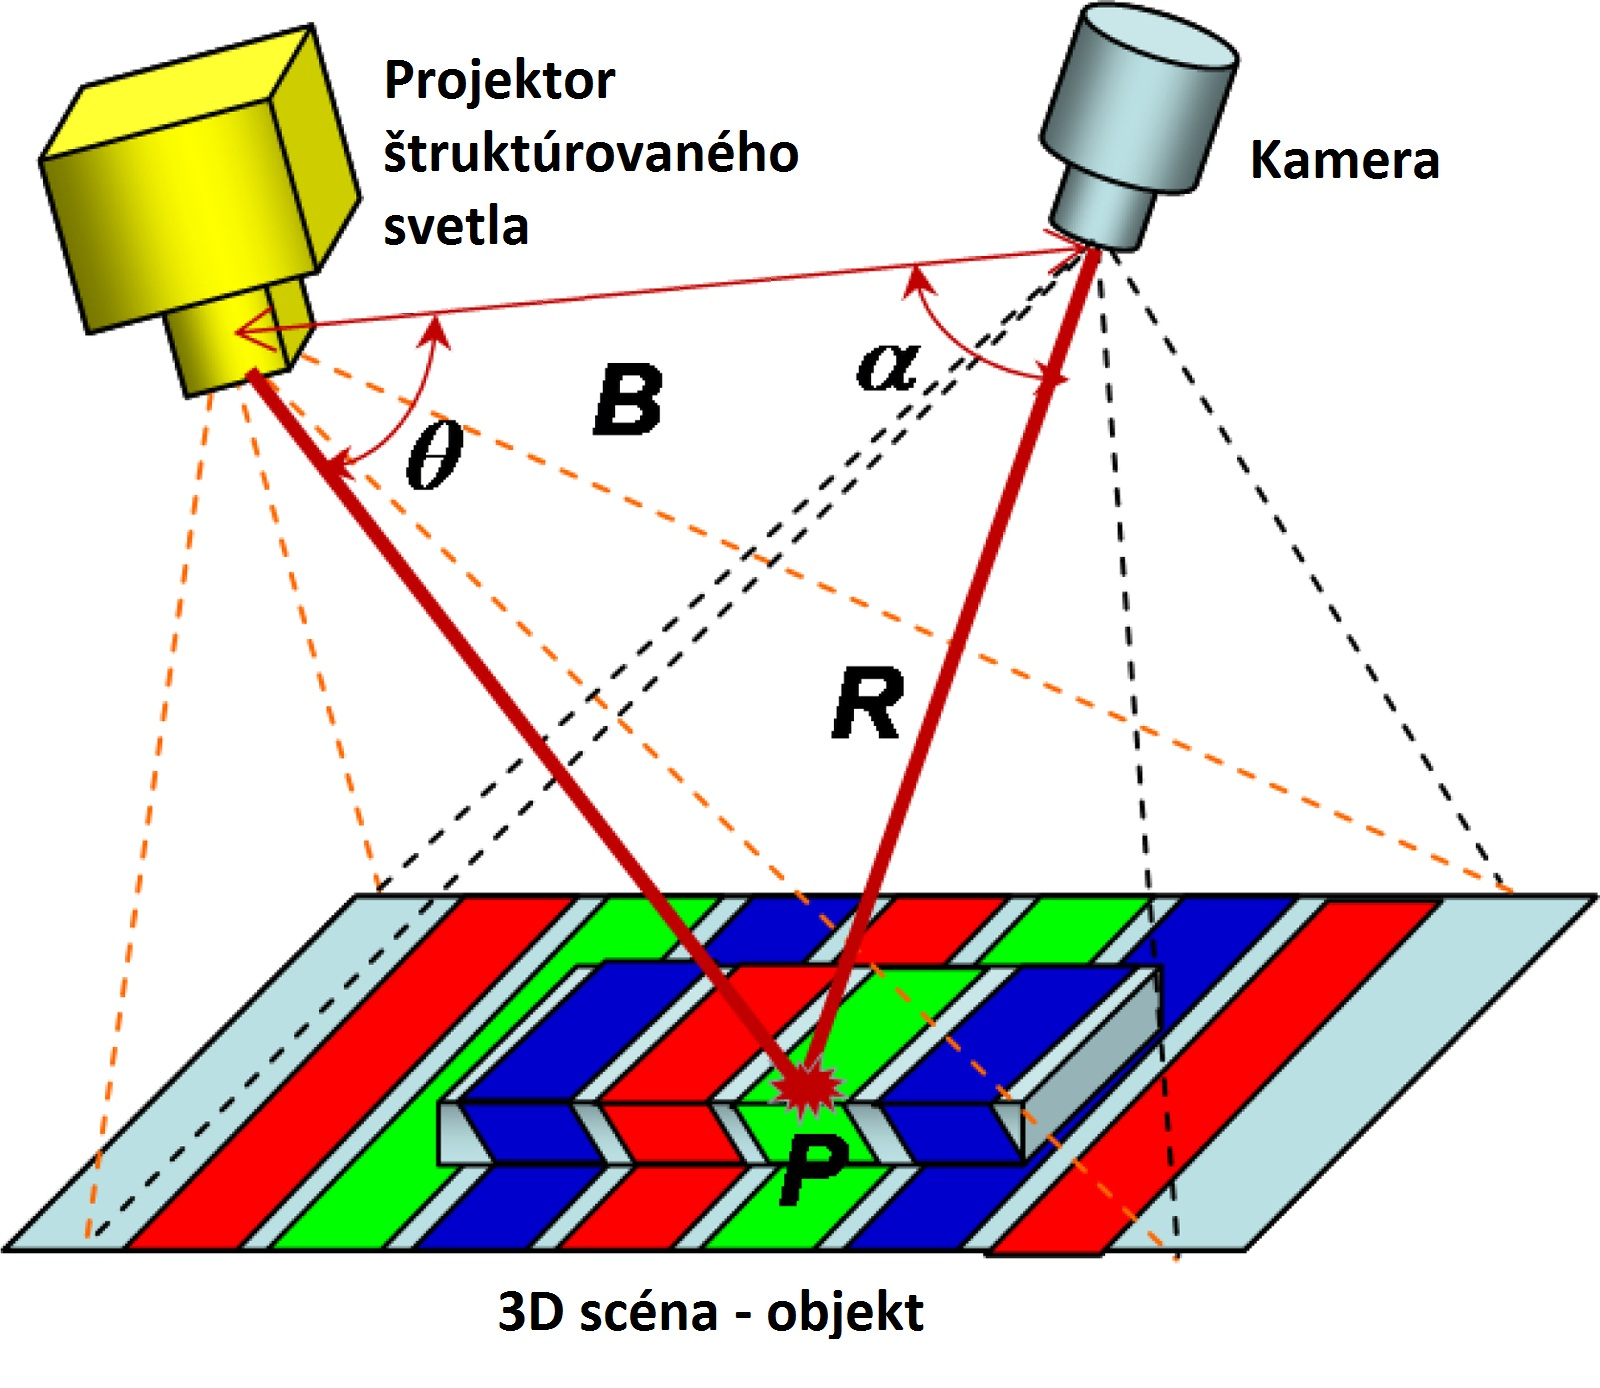
\includegraphics[width=0.5\textwidth]{figures/SLS.jpeg} 
	\caption{Princíp SLS kamery}
	\label{fig:sls}
\end{figure}

Na obr. \ref{fig:sls} je znázornený geometrický vzťah medzi projektorom, kamerou a snímaným povrchom. Tento vzťah je možné vyjadriť triangulačným princípom:
\begin{equation}
\label{eq1}
\begin{aligned}
R=B\frac{\sin\theta}{\sin\alpha + \theta}
\end{aligned}
\end{equation}

Kľúčom k 3D zobrazovaniu na báze triangulačnej techniky je správne priradiť zosnímaný bod
k projekčnému bodu (7). Na tento účel boli navrhnuté rôzne schémy, ktoré sa delia na:

\begin{itemize}
	\item \textbf{Sekvenčnú projekciu:} binárny kód, šedý kód, fázový posun, hybrid 
	\item \textbf{Priebežne meniacu projekciu:} dúhový kód, priebežne meniaci farebný kód 
	\item \textbf{Pásikový index:} farebne kódované pásy, segmentované pásy, De Bruijn, ...
	\item \textbf{Mriežkovaný index:} pseudo-náhodné binárne body, mini-vzor ako kód, ...
	\item \textbf{Hybridné metódy:} 
\end{itemize}

Hlavnou výhodou štruktúrovaného svetla je dosiahnutie vysokého priestorového rozlíšenia. Kamery pracujúce na tomto princípe nevyžadujú žiadnu špeciálnu úpravu na úrovni snímača. Akékoľvek rušenie je znázornené ako variácie v povrchu (7). Táto metóda snímania so sebou prináša tri problémy, ktoré vyplývajú z hlavnej požiadavky, a to dôležitosti svetla:


\begin{compactitem}
	\item Potreba konštantnej vlnovej dĺžky 
	\item Možné problémy spôsobené okolitými svetelnými podmienkami 
	\item Vzdialenosť limitovaná silou reflektora IR svetla
	\item Vznik multi-kamerovej interferencie
\end{compactitem} 
\vline

Konštantná vlnová dĺžka je zabezpečená malým Peltierovým článkom, slúžiacim na udržiavanie nemennej teploty laserovej diódy. Takým spôsobom je zabezpečená stabilná výstupná vlnová dĺžka, vzhľadom na zmeny teploty a výkonu. Osvetlenie okolitého prostredia je problémom, ktorý je možné zmierniť využitím filtra, ktorý prepúšťa iba IR frekvenčné pásmo. Avšak kamera nedokáže fungovať správne na miestach osvetlených slnečným žiarením. Preto je využívanie kamier na princípe štruktúrovaného svetla výhodnejšie využívať v interiéri (8).

\subsection{TOF snímače}
\label{sec:tof}
Kamery pracujúce na princípe \textit{Time of Flight} (TOF) produkujú hĺbkový obraz, ktorého každý pixel kóduje vzdialenosť od zodpovedajúceho bodu snímanej scény pomocou merania fázového oneskorenia infračerveného svetla. Kamery obsahujú zdroj infračerveného svetla a senzor, ktorý zachytáva odrazené svetlo. Taktiež sú často kombinované s RGB snímačom, ktorý dokáže zachytiť farebnú textúru snímanej scény. Infračervené svetlo je modulované harmonicky sínusovým signálom alebo impulzne. V praxi sa viac využíva impulzná modulácia, pretože je ľahšia na realizáciu a spracovanie. Obr.\ref{fig:tof_principle} popisuje princíp detekcie hĺbky TOF senzorom so sínusovou moduláciou.

\begin{figure}[h]
	\centering
	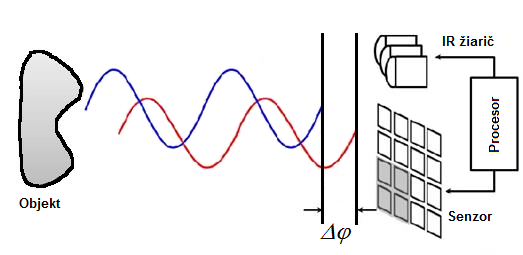
\includegraphics[width=0.7\textwidth]{figures/tof_principle.png} 
	\caption{Princíp činnosti TOF senzorov}
	\label{fig:tof_principle}
\end{figure}

Infračervené svetlo s moduláciou je vyžiarené z emitora, po dopade na objekt sa odrazí a spätne dopadá s fázovým oneskorením do senzora (10). Hĺbka je vypočítavaná podľa rovnice 3.2.
\begin{equation}
\label{eq2}
\begin{aligned}
Depth=\frac{c}{2}\frac{\Delta \varphi}{2 \pi f}
\end{aligned}
\end{equation}

Pri impulznej modulácii môže byť emitované svetlo sekvenčne alebo kontinuálne (11). Na Obr. 3.3 je znázornený princíp impulznej sekvenčej modulácie, kde je svetelný zdroj rozsvietený na krátky čas (Δt) a odrazená energia je prerozdelená na každý pixel paralelne pomocou dvoch fázových okien C1 a C2 s rovnakým trvaním Δt. Elektrické náboje, ktoré sa nahromadili počas týchto vzoriek, Q 1 a Q 2 , sú merané a použité na výpočet vzdialenosti pomocou vzťahu 3.3:

\begin{equation}
\label{eq3}
\begin{aligned}
Depth=\frac{c}{2}\cdot\Delta t \left( \frac{Q_2}{Q_1 + Q_2}\right) 
\end{aligned}
\end{equation}

\begin{figure}[H]
	\centering
	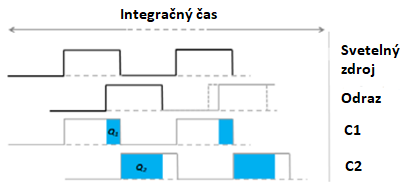
\includegraphics[width=0.65\textwidth]{figures/tof_principle_a.png} 
	\caption{Sekvenčná impulzná mdulácia TOF senzora}
	\label{fig:tof_principle_a}
\end{figure}

Metóda s použitím kontinuálnej vlny obsahuje viac vzoriek pre jedno meranie, pričom každá vzorka je posunutá s fázovým oneskorením o 90 stupnov. Meranie fázového rozdielu medzi vyžarovanými a odrazenými IR vlnami je zabezpečené prepočtom vzdialenosti od objektu na základe vzťahu 3.4 medzi štyrmi rôznymi hodnotami elektrického náboja.

\begin{figure}[H]

	\centering
	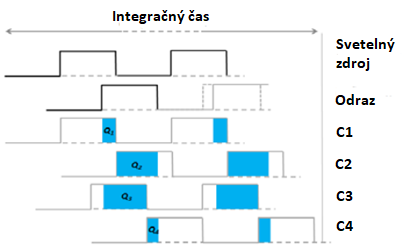
\includegraphics[width=0.65\textwidth]{figures/tof_principle_b.png} 
	\caption{Kontinuálna impulzná modulácia TOF senzora}
	\label{fig:tof_principle_b}

\end{figure}

Pomocou tejto techniky je vypočítaný fázový uhol $\Delta \varPhi$ medzi osvetlením a odrazom. Tento fázový posun je následne prepočítaný na hĺbku.

\begin{equation}
\label{eq4}
\begin{aligned}
\Delta \varphi=\tan^{-1} \left( \frac{Q_3 - Q_4}{Q_1-Q2} \right) 
\end{aligned}
\end{equation}

K spresneniu merania a eliminácii vplyvu akejkoľvek konštanty posunutia od merania sa z
prijatých odrazov počíta amplitúda intenzity A 3.5 a ofset B 3.6:

\begin{equation}
\label{eq5}
\begin{aligned}
A=\frac{\sqrt{\left(Q_1 - Q_2\right)^2 + \left(Q_3 - Q_4\right)^2 }} {2} 
\end{aligned}
\end{equation}

\begin{equation}
\label{eq6}
\begin{aligned}
B=\frac{Q_1 + Q_2 +Q_3 + Q_4}{4} 
\end{aligned}
\end{equation}

Amplitúda intenzity A a ofset B majú vplyv na presnosť merania hĺbky. Odchýlku merania hĺbky je možné aproximovať podľa vzťahu 3.7:

\begin{equation}
\label{eq7}
\begin{aligned}
\sigma=\frac{c}{4\sqrt{2 \pi f}} \frac{\sqrt{A+B}}{c_d A}
\end{aligned}
\end{equation}

v nej modulačný kontrast c d opisuje ako efektívny zobrazovací kremík oddeľuje a zbiera fotoelektróny. Amplitúda intenzity A je funkciou optickej sily a offset B je funkciou okolitého svetla. Z tejto rovnice možno vyvodiť, že vysoká odrazená amplitúda, frekvencia vysokej modulácie a kontrast s vysokou moduláciou prispievajú k zvýšeniu presnosti. Vysoký offset na druhej strane môže viesť k sýtosti a zníženiu presnosti. Snímače TOF s vysokou odchýlkou všeobecne prinášajú vyššiu presnosť (12). Hlavnou výhodou TOF kamier je používanie iba jedného pohľadu pri výpočte hĺbky, vďaka čomu sú zachované ostré hrany objektov a redukovaná prítomnosť otvorov vo výslednom obraze, pričom je zanechaná vysoká presnosť údajov. Hustotu nameraných dát je možné ovplyvniť počtom meraní. Výhodou je aj to, že okolité osvetlenie už nevplýva na zaznamenávanie obrazu, pretože nedochádza k ovplyvňovaniu frekvencie vyžarovaného svetla. K ďalším kladným vlastnostiam patrí vysoký dynamický rozsah a absencia cenovo náročných materiálov v zariadení. Medzi nevýhody kamier s TOF zaraďujeme nižšiu kvalitu priestorového rozlíšenia, zapríčinenú extra spracovaním na úrovni snímača, a taktiež náchylnosť na pohybové artefakty pri viacnásobnom počte záberov. Pri kamere využívajúcej TOF je potrebné vopred vedieť rýchlosť šírenia signálu v danom prostredí. Namerané výsledky sú závislé aj od materiálu meraného subjektu. Pri nevhodnom materiáli môže dochádzať k niekoľkonásobnému odrazu. Negatívne vlastnosti TOF sa prejavujú prevažne na okrajových pixloch (13)

\section{Mračno bodov a 3D povrch}

Pri reprojekcii 3D priestoru z 2D obrazu sa často používa technológia mračien bodov (Point Cloud). Základnou jednotkou mračna bodov je dátový bod, ktorý v sebe ukladá informáciu o polohe (x,y,z) v 3D priestore. Dátový bod môže v sebe uchovávať aj iné informácie ako napríklad farbu, jas, normálový vektor a podobne. Takéto mračno bodov má veľké využitie v priemyselných 3D CAD modeloch, pri metrológií a inšpekcií kvality a v iných sférach, kde sa vizuálne prezentujú 3D objekty. Výhodou oproti 2D zobrazovaniu je, že 3D model dokáže poskytnúť presnú geometrickú a lepšiu vizuálnu informáciu pre užívateľa.

\begin{figure}[!h]
	\centering
	\begin{subfigure}[b]{0.45\textwidth}
		\centering
		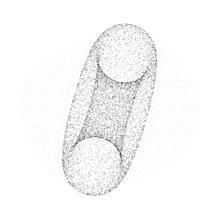
\includegraphics[width=0.7\textwidth]{figures/point_cloud_a.png}
		\caption{}
		\label{fig:point_cloud:a}
	\end{subfigure}
	\begin{subfigure}[b]{0.45\textwidth}
		\centering
		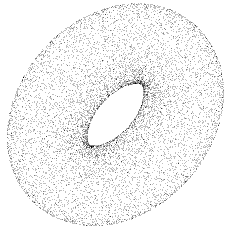
\includegraphics[width=0.7\textwidth]{figures/point_cloud_b.png}
		\caption{}
		\label{fig:point_cloud:b}
	\end{subfigure}
	\caption{Mračno bodov torusu pri rozdielných pohľadoch}
	\label{fig:point_cloud}
\end{figure}


Prevod mračna bodov na 3D povrch je realizovaný pomocou rekonštrukcie povrchu (\textit{surfacere construction}). Medzi známe rekonštrukčné metódy patrí Ball-Pivoting a  Poissonova rekonštrukcia, kde sú dátove body transformované do siete. Polygónová sieť je zložená z vertexov (vertices), hrán (edges) a masiek (faces), taktiež definuje tvar polyhedrálneho objektu v 3D grafike. Masky sa zvyčajne skladajú z trojuholníkov, štvorhranov a iných jednoduchých konvexných polygónov. Volumetrické siete explicitne reprezentujú povrch aj objem štruktúry, pričom polygónová sieť reprezentuje iba povrch. Objekty vytvorené z polygónov musia ukladať rôzne typy elementov. To zahrňa vertexy, hrany, masky, polygóny a povrchy. Veľakrát sú polygóny transformované na trojuholníky.

\begin{figure}[h]

	\centering
	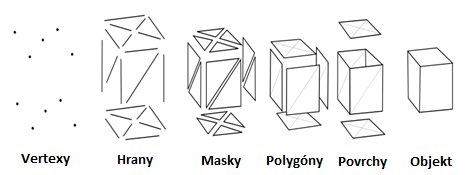
\includegraphics[width=0.7\textwidth]{figures/vertex_edge_polygon.png} 
	\caption{Elementy používané pri 3D spracovaní a modelovaní objektov }
	\label{fig:vertex_edge_polygon}

\end{figure}

\begin{description}[leftmargin=*,labelsep=5.8mm, font=$\bullet$~\normalfont\scshape\color{black!20!black}]
	\item[Vertex] Dátový bod, informácia o polohe poprípade farbe a normále 
	\item[Hrana] Spojenie medzi dvomi vertexmi 
	\item[Maska] Polygón zložený z najbližších hrán
	\item[Povrch] Skupina polygónov, ktorá vytvára povrch objektu.
\end{description}

\newpage
\section{Spájanie a registrácia mračien bodov}

Bodová registrácia tiež známa ako bodová zhoda je proces, pri ktorom sa hľadá priestorová transformácia zarovnávajúca dve mračná bodov. Účelom transformácie je zlúčenie viacerých mračien do jedného konzistentného modelu. Mračná môžu byť získané rôznymi typmi snímačov a rôznymi spôsobmi. Niektoré typy snímačov boli opísané v kapitole \ref{sec:rgbd:principles}. Pre získanie priestorovej transformácie existuje viacero algoritmov, ktoré sú opísané nižšie.


\subsection{Problematika registrácie mračien bodov}

Problematika registrácie mračien bola opísaná v práci „Robust Point Set Registration Using Gaussian Mixture Models„ autormi Bink Jian, Baba C. Verumi. Nech $\left\lbrace M, S \right\rbrace $ sú dva konečné mračná bodov v konečne-rozmernom reálnom vektorovom priestore. $M$ označuje pohyblivý modelový súbor a $S$ označuje statickú scénu. Obe množiny sa označujú ako podmnožiny konečno-priestorového vektora $\textbf{R}_{\textbf{d}}$ a môžu mať rozdielne veľkosti. Spoločným približovaním sa (registráciou) bodových množín $M$ a $S$ je možné odhadnúť mapovanie z $\textbf{R}_\textbf{d}$ do $\textbf{R}_\textbf{d}$ , čo prináša najlepšie zarovnanie medzi transformovanou a statickou sadou bodov. Transformačný model môže byť zapísaný ako $\textbf{T(M)}$ alebo $\textbf{T(M, $\theta$)}$, kde $\theta$ predstavuje optimalizačný parameter. Pri konvergencii bodov $M$ a $S$ je žiadané, aby vzdialenosť medzi zhodnými bodovými súbormi bola čo najmenšia. To je však bez vyskúšania všetkých transformácií ťažké, takže stačí lokálne minimum. Funkcia vzdialenosti medzi transformovaným dátovým setom a scénou $S$ je daná niektorou z funkcií $dist$. Jednoduchým spôsobom je výpočet štvorca euklidovskej vzdialenosti pre každý pár bodov:

\begin{equation}
\label{eq8}
\begin{aligned}
dist\left(T\left(M\right),S\right)=\sum_{m\epsilon T\left(M\right)} \sum_{s\epsilon S} \left(m-s\right)^2
\end{aligned}
\end{equation}

Táto funkcia je náchylná voči šumovým dátam. Robustnosť $g$ sa môže docieliť M-estimátorom, ktorý dokáže odfiltrovať extrémne hodnoty (17):

\begin{equation}
\label{eq9}
\begin{aligned}
dist_{robust}\left(T\left(M\right),S\right)=\sum_{m\epsilon T\left(M\right)} \sum_{s\epsilon S} g\left(m-s\right)^2
\end{aligned}
\end{equation}

\subsection{Spôsoby registrácie mračien bodov}

Spôsoby registrácie môžeme rozdeliť do dvoch kategórií. Prvou je pevná (rigid) druhá pružná (non-rigid) registrácia. Pri rigidnej registrácií sa používajú rotačné a translačné transformácie k namapovaniu jedného bodu na druhý. Táto transformácia je definovaná tak, že nemení vzdialenosť medzi dvoma bodmi. V zriedkavých prípadoch môže byť bodový súbor tiež zrkadlový. Pružná registrácia vzhľadom na dva bodové súbory prináša transformáciu, ktorá mapuje jeden bod nastavený na druhý. V transformáciách sú zahrnuté afinné transformácie, ktoré zahŕňajú aj nelineárne transformácie. Ak sú známe vlastné modifikácie množiny bodov, nelineárna transformácia môže byť parametrizovaná vlastnými hodnotami.\newline

\textbf{Bodové registračné algoritmy}

K bodovej registrácií sa používajú algoritmy, ktoré riešia všeobecnejší problém s porovnávaním grafov. Avšak výpočtová zložitosť zvykne byť vysoká a obmedzená na rigidné registrácie.\newline


\textbf{Interative closest point}
ICP algoritmus je používaný na minimalizáciu rozdielu medzi dvoma mračnami bodov. Využíva sa na rekonštrukciu 2D a 3D povrchov, lokalizáciu robotov a podobne. Vykonáva rigidnú registráciu interačným spôsobom za predpokladu, že každý bod v M korešponduje s najbližším bodom v S. V algoritme sa hľadá transformácia T pomocou metódy najmenších štvorcov.

\begin{figure}[h]

	\centering

	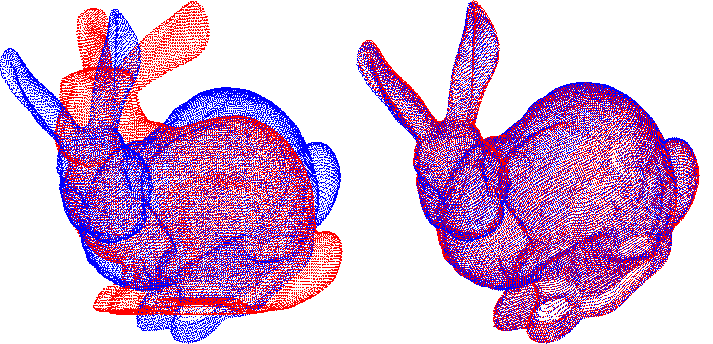
\includegraphics[width=0.7\textwidth]{figures/icp_principle.png} 

	\caption{Ukážka registrácie mračien}
	\label{fig:icp_principle}

\end{figure}
\newpage
\textbf{Robustné párovanie bodov}

Túto metódu (RPM) zaviedli Gold a kolektív (19). Táto metóda pracuje na zašumených 2D alebo 3D bodových setoch, ktoré môžu mať rozličné veľkosti a môžu sa líšiť pri voľných transformáciách. Pomocou kombinácie optimalizačných techník ako „deterministic annealing“ a „softassing“ , ktoré boli objavené pri rekurentných neurónových sieťach, sú analógové objektové funkcie popisujúce problémy minimalizované. Zatiaľ čo v ICP je korešpondencia vytvorená najbližším heuristickým binárnym systémom, RPM používa mäkkú korešpondenciu bodov. To znamená, že korešpondencia bodov môže byť ľubovoľná v rozmedzí 0 a 1. Zhoda v RPM je vždy jedna k jednej, čo pri ICP metóde nie je zabezpečené. Ak $m_i$ je i-ty bod množiny $M$ a $s_j$ je j-ty bod množiny $S$, tak matica zhody $\mu$ je definovaná ako:

\begin{equation}
\label{eq10}
\begin{aligned}
\mu_{ij}=
\begin{cases}
1, & \text{ak bod}\ m_i\ \text{korešponduje s bodom}\ s_j \\
0, & \text{v inom prípade}
\end{cases}
\end{aligned}
\end{equation}

Riešením je nájsť afinnú transformáciu T , pri ktorej bude matica μ vykazovať najvyššiu zhodu (19). Znalosť optimálnej transformácie umožňuje ľahko určiť maticu zhody a naopak. Robustným párovaním bodov je možné určiť obe veci súčasne. Transformácia sa môže rozložiť na translačný vektor a transformačnú maticu.

\begin{equation}
\label{eq11}
\begin{aligned}
T\left(m\right)=\bar{A}m+\bar{t}
\end{aligned}
\end{equation}

Matica \textbf{A} sa skladá zo štyroch samostatných parametrov $\left\lbrace a, \theta, b, c \right\rbrace$, ktoré spôsobujú zmenu veľkosti, rotáciu, horizontálnu a vertikálnu geometrickú transformáciu.

Účelová funkcia je reprezentovaná rovnicou 3.12 pričom v nej platí podmienka 3.13:

\begin{equation}
\label{eq12}
\begin{aligned}
cost=\sum_{j=1}^{N}\sum_{i=1}^{M} \mu_{ij} \Arrowvert s_j - \boldsymbol{t} - \boldsymbol{Am_i} \Arrowvert^2 + \boldsymbol{g\left(A\right)} -\alpha \sum_{j=1}^{N}\sum_{i=1}^{M} \mu_{ij}
\end{aligned}
\end{equation}

\begin{equation}
\label{eq13}
\begin{aligned}
\forall j \sum_{i=1}^{M} \leq 1, \forall i \sum_{j=1}^{N} \mu_{ij} \leq 1, \forall ij \mu_{ij} \in \left\lbrace 0,1 \right\rbrace 
\end{aligned}
\end{equation}

Parameter $\alpha$ ovplyvňuje funkciu k silnejšej korelácii. Funkcia $g\left(A\right))$ slúži na reguláciu afinnej transformácie penalizovaním veľkých hodnôt transformovaných komponentov. Pre niektoré regulačné parametre $\gamma$ platí $g\left(A\left(a, \theta, b, c\right)\right) = \gamma \left(a^2 + b^2 + c^2 \right)$. Táto metóda RPM optimalizuje hodnotovú funkciu použitím „Softassign“ algoritmu.

\textbf{Korelácia kernelu}

Metóda korelácie kernelu (KC) je oproti ICP metóde odolnejšia vočí zašumeným dátam. Na rozdiel od ICP, v tejto metóde každý bod scény uvažuje s modelovým bodom. Ide o viacnásobne prepojujúcu registráciu (18). Pre niektoré funkcie kernelu $K$ je KC dvoch bodov $\chi_i$ a $\chi_j$ definovaná nasledovne:

\begin{equation}
\label{eq14}
\begin{aligned}
KC\left(\chi_i,x_j\right)=\int K\left(\chi,\chi_i\right) \cdot K\left(\chi,\chi_j\right) dx 
\end{aligned}
\end{equation}

Funkcia K zvolená pre bodovú registráciu je typický symetrický a nenegatívný kernel. Zvyčajne je používaný Gaussov kernel pre svoju jednoduchosť, avšak časté sú aj \textit{Epanechnikov} a \textit{tricube} kernel (18). Korelácia kernelu celej množiny bodov χ je definovaná ako súčet korelácií kernelu každého bodu v množine s každým ďalším bodom v množine.


\begin{equation}
\label{eq15}
\begin{aligned}
KC\left(\chi\right) = \sum_{i\ne1} KC\left(\chi_i,\chi_j\right)=2\sum_{i<j} KC\left(\chi_i,\chi_j\right)
\end{aligned}
\end{equation}

Hodnota $KC$ množiny bodov je proporcionálna v rámci konštantného faktora logaritmu informačnej entropie. $KC$ je v podstate mierou kompaktnosti bodu, ktorý je triviálne nastavený. Ak by sa všetky body nachádzali v jednom mieste, $KC$ by nadobudol veľkú hodnotu. Účelová funkcia ($cost$) dátovej množiny pre určité transformačné parametre $\theta$ je definovaná nasledovne :

\begin{equation}
\label{eq16}
\begin{aligned}
cost\left(S,M,\theta\right)= - \sum_{m\in M} \sum_{s\in S} KC \left(s, T\left(m, \theta \right)\right)
\end{aligned}
\end{equation}

Niektoré algebrické manipulácie sú opísané rovnicou 3.17:

\begin{equation}
\label{eq17}
\begin{aligned}
KC\left(S\cup T\left(M,\theta\right)\right) = KC\left(S\right) + KC\left(T \left(M, \theta \right)\right) - 2cost\left(S,M,\theta \right)
\end{aligned}
\end{equation}

Výraz je zjednodušený tým, že sa pozoruje $KC\left(S\right)$ nezávisle od $\theta$. Ak sa ešte uvažuje s rigidnou registráciou, $KC\left(T \left(M, \theta \right)\right)$ je tým pádom invariantný voči zmene $\theta$, pretože Euklidovská vzdialenosť medzi párom bodov sa pri rigidnej transformácií nemení. Tým pádom je rovnicu 3.17 možné prepísať na 3.18:

\begin{equation}
\label{eq18}
\begin{aligned}
KC\left(S\cup T\left(M,\theta\right)\right) = c - 2cost\left(S,M,\theta \right)
\end{aligned}
\end{equation}


Estimácia hustoty kernelu je neparametrický spôsob odhadovania hustoty pravdepodobnosti náhodnej premennej. Odhad hustoty kernelu je základným problémom vyhladzovania údajov na základe dátovej vzorky. Jej definícia pre tento prípad je znázornená v rovniciach 3.19 a 3.20.

\begin{equation}
\label{eq19}
\begin{aligned}
P_M\left( \chi,\theta\right)=\frac{1}{M}\sum_{m\in M} K\left(\chi,T\left(m,\theta\right)\right)
\end{aligned}
\end{equation}

\begin{equation}
\label{eq20}
\begin{aligned}
P_S\left( \chi\right)=\frac{1}{N}\sum_{s\in S} K\left(\chi,s\right)
\end{aligned}
\end{equation}

Účelovú funkciu následne možno dokázať ako koreláciu odhadov hustoty kernelu.

\begin{equation}
\label{eq21}
\begin{aligned}
cost\left(S,M,\theta\right)= - N^2 \int_{\chi} \left(P_M P_s\right)
\end{aligned}
\end{equation}

Po získaní hodnotovej funkcie algoritmus používa zostup gradientu, čo je iteračný optimalizačný algoritmus prvého radu na zistenie minimálnej funkcie. Ním sa nachádza optimálna transformácia. Z dôvodu výpočtovej náročnosti sa používa diskrétna verzia funkcie 3.18 cost. Oproti ICP algoritmu KC metóda nepotrebuje nájsť najbližšieho suseda a tým pádom je ľahšia na implementáciu. Taktiež je menej náchylná na šum v dátach (18).

